% Two maps of Congress: the paper cut to six pages. Full draft written 25 Nov 2026 by Anas with Claude in the course's
% PNAS template (SGAI.zip); pruned 25 Nov 2026 by Martin with Claude from the group's printed comments
% (../v2_comments_SGAI_PAPER.pdf) and ../TEXT_TAKEAWAYS.md. Every paragraph has a % line naming its source.
% Nothing here is a new analysis; every number comes from an existing result file (see the % lines).
\documentclass[9pt,twocolumn,twoside]{pnas-new}
\articletype{Political Sciences}
\templatetype{pnasresearcharticle}

% Less whitespace around figures: tighter gaps between floats and text, a shorter gap to the caption, and
% float fractions that let text fill the rest of a column instead of leaving a float alone on a page.
\setlength{\textfloatsep}{8pt plus 2pt minus 2pt}
\setlength{\dbltextfloatsep}{8pt plus 2pt minus 2pt}
\setlength{\floatsep}{6pt plus 2pt minus 2pt}
\setlength{\dblfloatsep}{6pt plus 2pt minus 2pt}
\setlength{\intextsep}{6pt plus 2pt minus 2pt}
\captionsetup[figure]{skip=4pt}
\renewcommand{\topfraction}{0.95}
\renewcommand{\dbltopfraction}{0.95}
\renewcommand{\textfraction}{0.05}
\renewcommand{\floatpagefraction}{0.9}
\renewcommand{\dblfloatpagefraction}{0.9}

\begin{document}

\title{Two maps of Congress: the US House is less divided in whom its members name than in whom they work with}

\author[a]{Anas Mir}
\author[a]{Martin M{\o}llenhus}
\author[a]{Diego A. Mijares}
\affil[a]{Technical University of Denmark, 02805 Social Graphs and Interactions}

\leadauthor{Mir}

% Diego's significance statement, cut to three sentences for a reader outside the field (course rule).
\significancestatement{Divisions in the US Congress are usually read from votes or vocabulary. We read them from
whom members name: on the House floor, members name colleagues across the aisle more often than they cosponsor
with them, mostly to give them credit, and in press releases the members whose seats are at risk name the other
party most, mostly as partners. How divided Congress looks depends on the record read, and a named partner can be
checked against the legislative record in a way the word ``bipartisan'' cannot.}

% Contributions: rewritten 25 Nov from the owners in WORK_AND_DEADLINES.md section 2 (M1-M8, A1-A6, D1-D5, S1-S2).
\authorcontributions{M.M. built the shared name matcher, the floor and working maps, their null models and community
analysis, and the null for cited bills, made Figure 1, and wrote the Results and Methods on the two maps. A.M.
built the press-release collector, collected the 55,023 releases and matched them to members and bills, measured
district lean, ran the exposure analysis and its checks, the home map and the analysis of ``bipartisan'' releases,
made Figures 3 and 4, and wrote the Results and Methods on press releases. D.A.M. wrote the labelling rules, coded
the 100 mentions, measured the matcher's precision and the speaker attribution, built the text classifier, compiled
the literature and the record of AI use, made Figure 2, and wrote the Results and Methods on what mentions do.
M.M. and A.M. second-coded the mentions; D.A.M. and M.M. wrote the Introduction and Discussion; all authors revised
the whole paper. Code and text were first drafted with Claude (Anthropic) and then rewritten and extended by the
authors (Methods, AI use).}
\authordeclaration{The authors declare no competing interest.}
\correspondingauthor{}

\keywords{Congress $|$ polarization $|$ networks $|$ floor speech $|$ press releases}

% Abstract: Nature summary-paragraph structure, 150 words (course). Press releases weighted as in the Results.
\begin{abstract}
Divisions in the US Congress are usually measured from votes or vocabulary, and both show two camps. Yet division
depends on the record read, and it is unknown whether members are as divided in whom they name as in whom they work
with. Here we show that in the 119th House (2025--2026), the network of who names whom on the floor is less divided than the cosponsorship network of the same 450 members: at equal size, 38.7\% of
naming ties cross the party line, against 28.6\%. Debate procedure accounts for about two thirds of the naming
network's division, and cross-party names are mostly credit (69\%), rarely disagreement (7\%). In 55,023 press
releases, members in electorally close seats name the other party more often than members in safe seats, mostly as
partners, though seat and moderation cannot be separated. A name, unlike a slogan, can be checked against the
legislative record.
\end{abstract}

\dates{Draft of 25 November 2026.}

\maketitle
\thispagestyle{firststyle}
\ifthenelse{\boolean{shortarticle}}{\ifthenelse{\boolean{singlecolumn}}{\abscontentformatted}{\abscontent}}{}

% Page 1: text in one wider block, Significance box on the right (template). Page 1 ends at the \Parasplit below.
% When text before it changes, move \Parasplit to the last word on page 1 (or use \Endparasplit after a paragraph
% that ends exactly at the bottom of page 1).
\Firstpage

% ================================================================ INTRODUCTION
% Diego and Martin's introduction (report/sections/introduction.tex). 25 Nov: other studies' claims attributed to
% their authors (comment 3), roll-call votes and exposed seats defined, the preview cut to one sentence.

\dropcap{T}he United States Congress is usually described as two camps, and most ways of measuring it agree. Members
of the two parties vote apart, and since the early 1990s they have used increasingly different words
\cite{gentzkow2019}. Networks built from who signs whose bills show the same split, with ties between the parties
growing rarer and more hostile over four decades \cite{neal2020}.

How deep the split looks depends, however, on which record is read. Harbridge finds that between 1973 and 2004
bipartisan agreement fell in roll-call votes, the recorded votes in which each member's yes or no is published,
while it stayed far more stable in cosponsorship, and traces the difference to party leaders choosing which bills
reach a vote \cite{harbridge2015}. Green and colleagues find the parties distinguishable in every channel of
communication, but more so before national audiences than local ones \cite{green2024}. Division, on this evidence,
is a property of the measurement as well as of the institution.

Members also have reasons to manage how divided they appear. In survey experiments, voters with weak party
attachments rewarded a bipartisan image \cite{harbridge2011}, and Grimmer describes what members tell constituents
as a strategic presentation of their work \cite{grimmer2013}. That presentation need not match the work: Westwood
finds that floor speeches calling a bill bipartisan mostly concern bills with trivial support from the other party,
and that a member's bipartisan rhetoric is unrelated to their bipartisan votes \cite{westwood2022}. A word such as
``bipartisan'' costs nothing to say. A name points at a specific colleague, and what is said about that colleague
can be read.

We therefore compare three records of the same members of the 119th House (2025 to 2026). The first is the
cosponsorship network \cite{fowler2006}: two members are tied when one signs a bill the other sponsors. The second
is, to our knowledge, new: two members are tied when one names the other in a floor speech. Both are networks on the
same members, so the same measures of party division and the same null models apply to each. The third is the
members' own press releases, written for voters at home. If showing bipartisanship pays off with some voters, the
members in electorally exposed seats, whose district leans only slightly or not at all towards their own party,
should name the other party most there.

Whether naming is more or less partisan than working cannot be guessed in\Parasplit
advance: members might attack the other side in public and cooperate quietly, or display the few cross-party partners they have. We find that the floor map
is less divided than the working map, partly because of how debates are run, that cross-party names on the floor
are mostly credit, and that at home members in exposed seats name the other party more, mostly as partners.

% ================================================================ RESULTS
\section*{Results}

% ---------------------------------------------------------------- PART 1 (Martin)
% Source: Martin/results_part1.md (report/sections/from_martin_results.tex). Numbers: Martin/m3_table.csv,
% m3_random_draws.csv, m4_results.csv, m3b_state_null.csv, m5_table.csv, m5_committees/committee_table.csv.
% Figure 1: side caption (SCfigure*, sidecap is loaded by the class): 11.4 cm figure (Martin/m7_figure1.py --side).
\begin{SCfigure*}[0.5][t]
\centering
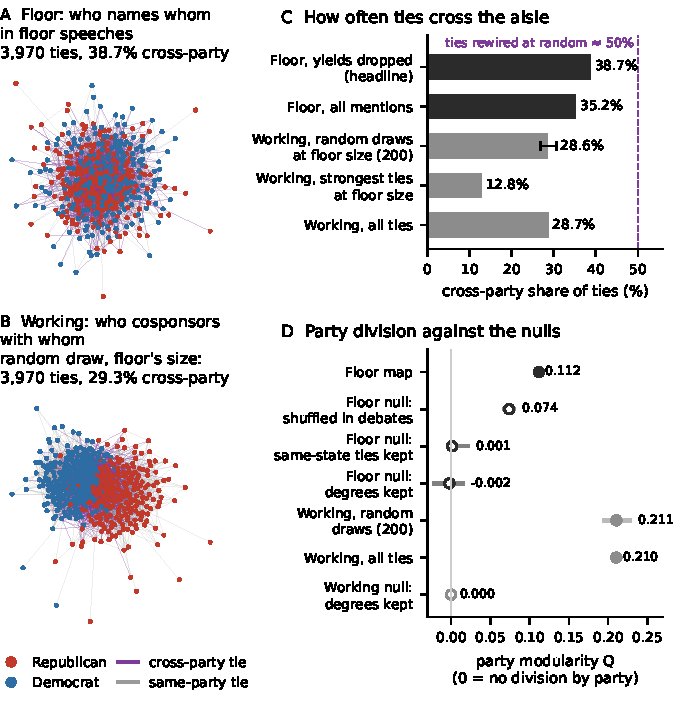
\includegraphics[width=11.4cm]{figures/figure1_side.pdf}
\caption{The House as two networks, January 2025 to November 2026. (\emph{A}) Floor map: members tied when one
names the other in a floor speech, yields of debate time left out. (\emph{B}) Working map: one random draw of
sponsor--cosponsor ties, thinned to the floor map's 3,970 ties. Red: Republicans; blue: Democrats; purple ties cross
the aisle; positions carry no meaning. (\emph{C}) Share of ties that cross the aisle; the bar for the random draws
spans 200 draws, and the dashed line is the level under random rewiring. (\emph{D}) Party modularity of each map
(filled) against its nulls (open; lines span the draws). The floor map is less divided than the working map at
every comparison, and more divided than every null.}
\label{fig:maps}
\end{SCfigure*}

\subsection*{The floor map is less divided than the working map}

We built two networks on the same 450 Republicans and Democrats. In the working map, two members are tied if one
cosponsored a bill or joint resolution that the other sponsored (46,513 ties). In the floor map, two members are
tied if one named the other in a floor speech, leaving out yields of debate time (3,970 ties from 8,469 mentions;
Methods). The share of ties that cross the aisle says how often a tie joins the two parties, not what the tie means;
that is the subject of the next section.

On the floor, 38.7\% of ties cross the aisle (Fig.~\ref{fig:maps}\emph{A} and \emph{C}). The floor map is about
twelve times sparser than the working map, so we compare it with working ties drawn at random at the same size.
Across 200 draws, 28.6\% of working ties cross the aisle (range 26.8\% to 30.6\%), and no draw comes within eight
points of the floor map (Fig.~\ref{fig:maps}\emph{B} and \emph{C}). Party modularity agrees: 0.112 for the floor map
against 0.211 (0.193 to 0.230) for the draws (Fig.~\ref{fig:maps}\emph{D}). Leaving out yields does not create the
gap: with yields kept, the floor map is at 35.2\% against 28.7\%. Members' strongest working partnerships are far
more partisan still: of the 3,970 pairs who share the most bills, 12.8\% cross the aisle.

% Comment 4 ("partly procedure. Meaning?"): the mechanism is now said in the sentence that names it.
Both maps are more divided than chance. If ties were rewired at random with every member keeping their number of
ties, about half would cross the aisle and modularity would be near zero in both maps (Fig.~\ref{fig:maps}\emph{C}
and \emph{D}). Part of the floor map's division comes from how debates are run: each debate has its own cast of
speakers and named members, often with a floor manager from each party, and that cast limits whom a speaker names.
Shuffling who is named only within each debate leaves a modularity of 0.074 (0.065 to 0.082 over 200 shuffles)
against 0.112 observed, so debates account for about two thirds of the floor map's division; the rest, members
naming their own side beyond what the debate forces, exceeds every shuffle. State delegations account for almost
none of it: keeping each member's same-state ties gives a modularity of 0.001 (at most 0.023).

The communities tell the same story. On the working map, the communities that the Louvain method finds are the two
parties (normalised mutual information with party, NMI, 0.83). On the floor map they cut across party (NMI 0.03,
against 0.29 for working draws of the same size): eight communities of 28 to 80 members, each holding both parties.
In seven of them one House committee is 3.0 to 7.9 times as common as in the House as a whole, among them
Appropriations (82\% of the community's members), Ways and Means (79\%) and Energy and Commerce (67\%); the eighth
gathers the party leaders. 44\% of floor ties join two members of the same committee, against 17.1\% when ties are
rewired at random, and so do 50\% of cross-party floor ties; in the working map the share barely exceeds chance
(22\% against 18.7\%). Much of the floor's cross-party naming runs within committees. A name can still be an attack
as easily as a thanks.

% ---------------------------------------------------------------- PART 2 (Diego)
% Source: report/sections/results.tex part 2 (Diego), Diego/d2_labelling/RESULTS.md, Diego/d5_classifier/results.txt.
\subsection*{Cross-party names on the floor are mostly credit}

To find out what the floor map's cross-party ties are, we read 100 floor mentions drawn at random, 75 between parties
and 25 within a party, and coded what the speaker was doing towards the named member (Methods). Of the cross-party
mentions, 69\% (95\% interval 58\% to 79\%) were agreeing: thanks to a bill's co-lead or to a committee's chair,
praise for joint work, support for the member's bill. 23\% (15\% to 33\%) were neutral references, such as the member
who introduced a bill. Only 7\% (3\% to 15\%) disagreed with the named member (Fig.~\ref{fig:labels}). None was
procedure: handing over debate time stays within a party (12\% of same-party mentions). Two human coders agreed on
82\% of the mentions (Cohen's $\kappa = 0.64$). A text classifier trained on these labels did not beat always
answering ``agreeing'' (73\% against 72\%), so we report the hand-labelled shares only.

The floor's cross-party ties are thus mostly acknowledgement, and they fit the committee communities: members thank
the managers and chairs they worked with. On the floor, though, procedure decides much of who meets whom. A press
release has no such script: the member chooses whom to name, and writes for the voters at home.

% Figure 2: Diego's figure and caption (Diego/d2_labelling/figure2.py --short, 4.4 cm tall).
\begin{figure}[t]
\centering
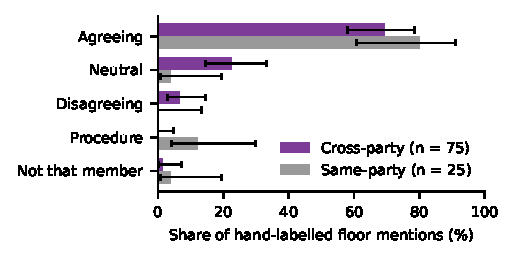
\includegraphics[width=8.7cm]{figures/figure2.pdf}
\caption{What floor mentions do. Share of 100 hand-labelled mentions in each code, for mentions between parties
(purple, $n = 75$) and within a party (grey, $n = 25$), with 95\% Wilson intervals. ``Not that member'': the matched
name referred to someone else. Cross-party mentions are mostly agreeing and rarely disagreeing; procedure appears
only within a party.}
\label{fig:labels}
\end{figure}

% ---------------------------------------------------------------- PART 3 (Anas)
% Source: Anas/results_part3.tex (report/sections/results_part3.tex). Numbers: Anas/a4/out/results.csv,
% member_shares.csv, leave_one_state_out.csv; check T a4/check_tone/scored.csv; check I a4/out/ideology_check.csv.
\subsection*{At home, members in exposed seats name the other party more}

If naming the other side is partly a message to voters, it should depend on which voters a member needs. We
collected 55,023 press releases posted by 412 members on their own websites between 3 January 2025 and 20 November
2026. For each of the 406 members with at least ten releases, we measured the share of releases that name a House
member of the other party who is neither a party leader nor a co-lead of a bill the release cites; a co-lead is named
because of the bill, not by choice. A seat is exposed when the district the member served leans toward their own
party by five points or less (Cook PVI 2025 \cite{cook2025pvi}), including seats that lean to the other party. 37
Republicans and 54 Democrats are exposed.

% Figure 3: Anas's figure (Anas/a4/figure3_column.py) and caption; the list of checks moved to Methods.
\begin{figure}[!t]
\centering
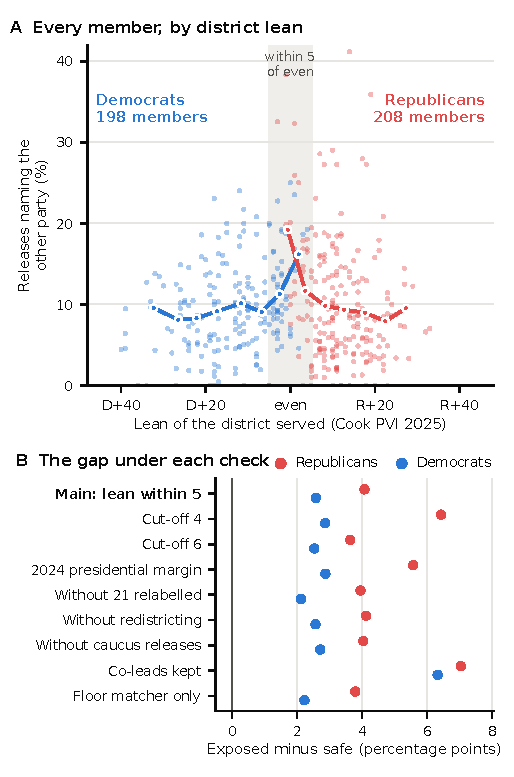
\includegraphics[width=8.7cm]{figures/figure3.pdf}
\caption{Members in exposed seats name the other party more often in their press releases. (\emph{A}) Each dot is
one of 406 members (53,664 releases): the share of their releases naming a House member of the other party who is
neither a party leader nor a co-lead of a cited bill, against the lean of the district they served (Cook PVI 2025).
Lines join the mean share in 5-point bands of lean (at least five members each); shading marks districts within five
points of even. (\emph{B}) Exposed minus safe mean share, by party, for the main definition (top) and for each check
fixed before the analysis (Methods). Every gap is positive with $p < 0.05$ (labels shuffled within party). The share
peaks in the closest seats and is nearly flat beyond them.}
\label{fig:home}
\end{figure}

Exposed Republicans named Democrats in 13.3\% of their releases, against 9.2\% for safe Republicans; exposed
Democrats named Republicans in 11.6\%, against 9.0\% (permutation $p = 0.004$ for each; Fig.~\ref{fig:home}). The two
gaps differ by 1.5 points ($p = 0.36$), too little to tell whether being in the president's party matters. The
difference sits in the closest seats: members whose district is even or leans to the other party named the other
party most (Republicans 19.2\%, $n = 8$; Democrats 14.2\%, $n = 10$), and beyond five points of lean the share is
nearly flat, between 7.9\% and 10.1\% (Fig.~\ref{fig:home}\emph{A}). Every check fixed before the analysis gives a
positive gap in both parties with $p < 0.05$ (Fig.~\ref{fig:home}\emph{B}); the gaps keep their sign when any one
state is left out, and widen to 7.0 and 6.3 points when co-leads count too.

% Check T (Anas). Kept as written: the printed comments praised its tone (comment 6).
A count of names says nothing about tone: an exposed member could name the other side to attack it. Three blind AI
readers, who did not see the seat, coded 60 of the counted names, 15 for each party and seat. 46 named a partner or
praised the member (77\%), 9 were neutral mentions such as a committee chair addressed in a letter, 4 were wrong
matches, and one criticised (a safe Republican on a Democrat's remarks). Exposed and safe seats did not differ in
criticism. At home, as on the floor, cross-party names are mostly acknowledgement.

% Check I (Anas), rewritten in three plain steps (comment 5).
Exposed members are also their party's moderates. DW-NOMINATE scores each member's ideology from their roll-call
votes: 22 of the 37 exposed Republicans and 27 of the 54 exposed Democrats are in their party's most moderate fifth,
and only 3 and 2 in the most extreme. Comparing exposed with safe members only within the same party and ideology
band leaves little of the gap: 1.1 of the 4.1 Republican points and 0.2 of the 2.6 Democratic points, neither
distinguishable from chance ($p = 0.39$ and $0.76$). This check may be too strict: if a close seat makes a member vote
more moderately, holding the voting score fixed also removes part of the seat's own effect. Our data therefore
cannot say whether the seat or the member's ideology drives the naming.

% Source: Anas/results_part3.tex (network paragraph); numbers a4/out/home_measures_centrality.csv, home_measures_null.csv,
% home_ties.csv, alpha_centrality.csv. The home map's community paragraph was cut on 25 Nov (DECISIONS G22).
\subsection*{Exposed members are the bridges of the home map}

Tying two members when one names the other in a release gives a third network, the home map, on the same 406
members. In both parties exposed members are its hubs. They are 22\% of members but send 35\% and receive 34\% of its
cross-party ties, and they are tied to 1.9 times (Republicans) and 1.5 times (Democrats) as many members of the other
party as safe members are (Holm-corrected $p = 0.001$ for each; Fig.~\ref{fig:homemap}\emph{B}). Exposed members tie
to each other only slightly more than their activity predicts: 10.7\% of cross-party ties join two exposed members,
against 10.2\% when ties are rewired with every member's number of ties kept ($p = 0.015$).

% Figure 4: Anas/a4/figure_home_map.py, full width so the purple cross-party ties stay visible (Martin, 25 Nov).
\begin{figure*}[!t]
\centering
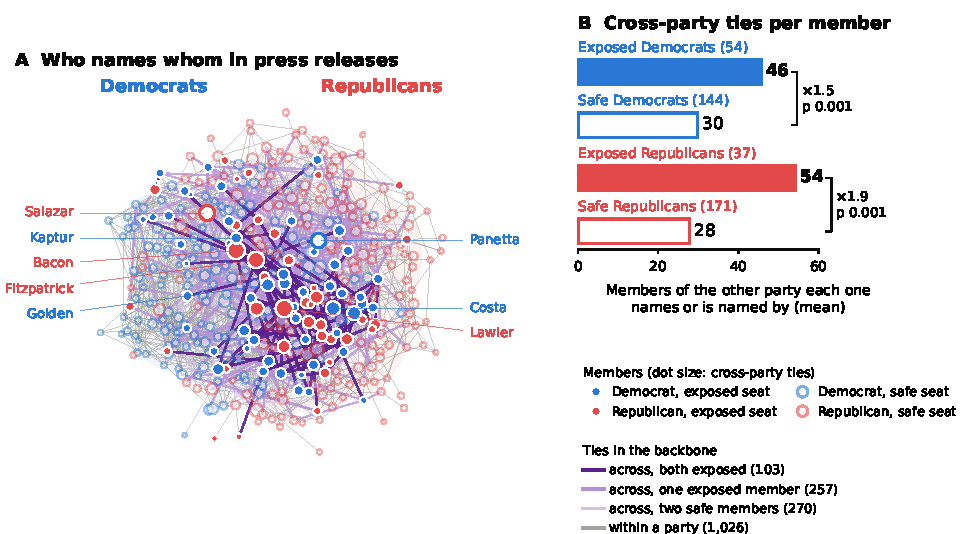
\includegraphics[width=17.8cm]{figures/figure4.pdf}
\caption{Who names whom in press releases. (\emph{A}) Each dot is one member ($n = 406$), placed by ForceAtlas2 on the
backbone of naming ties (disparity filter, $\alpha = 0.01$). Filled dots: exposed seats; hollow dots: safe seats; dot
size: number of cross-party ties. Purple lines cross the aisle, darkest between two exposed members; grey lines stay
within a party. Positions illustrate the network and are not a measurement. (\emph{B}) Members of the other party
each member names or is named by, on average: exposed members have 1.5 (Democrats) and 1.9 (Republicans) times as
many as safe members ($p = 0.001$, exposure shuffled within party, Holm-corrected over ten comparisons). Exposed
members of both parties sit where the two parties meet.}
\label{fig:homemap}
\end{figure*}

On the backbone, which keeps each member's strongest ties \cite{serrano2009}, the parties differ. Exposed
Republicans have 1.5 times the backbone ties of safe Republicans (Holm $p = 0.013$): they bridge by volume. Exposed
Democrats have no more backbone ties than safe Democrats but sit on more shortest paths than their ties predict (Holm
$p = 0.08$ at our backbone level, below 0.05 at every looser one): they bridge by position. We did not test why.

% Source: Martin's M6 paragraph (report/sections/from_martin_m6.tex; Martin/m6_results.csv) and Anas's A5 paragraph
% (Anas/results_part3.tex; a5/out/results.csv, a5/check/).
\subsection*{What members say at home mostly matches their record}

A name at home can be checked against the working map. Of the bills a member sponsored, those with an original
cosponsor from the other party were cited in that member's press releases more often than their other bills (52.7\%
against 45.1\%; 388 members, 10,125 bills; one-sided $p < 0.001$ when shuffling, within each member, which bills count
as cross-party). Most of the gap, however, separates co-led bills from solo bills: against bills co-led only by the
member's own party, cross-party bills are cited 3.5 points more often (52.6\% against 49.1\%, one-sided $p = 0.02$).
We cannot rule out that bipartisan bills are cited more because they more often pass.

The word ``bipartisan'' can be checked the same way. A quarter of the releases (13,744) call something bipartisan. In
64\% of them a House member of the other party is named or co-leads a cited bill, against 9\% of other releases (means
over 370 members). Three blind AI readers checked 30 releases of each kind: of those naming a member of the other
party, 28 named a partner and none an opponent; in those naming none, the word describes a bill, a vote or past
funding. Where Westwood found the floor's bipartisan rhetoric detached from votes \cite{westwood2022}, the word at
home mostly comes with a partner. Exposed Democrats back it with a partner more often than safe Democrats (63.0\%
against 56.7\%, $p = 0.012$); exposed and safe Republicans do not differ (72.1\% against 69.1\%, $p = 0.40$).

% ================================================================ DISCUSSION
% Diego and Martin's discussion (report/sections/discussion.tex), extended to part 3. 25 Nov: summary cut, the
% party-difference paragraph cut to one sentence, limits framed as what we were limited by (comment 7).
\section*{Discussion}

Drawn from the same members over the same two years, the House looks less divided in whom its members name than in
whom they work with, and the names across the aisle are mostly credit. At home the same holds: members name partners,
and when they call something bipartisan, a partner is mostly named or on a cited bill.

The result does not show that members cooperate more than cosponsorship suggests. A mention is a reference, made in a
setting where House procedure brings members of both parties into the same debates; that procedure accounts for about
two thirds of the floor map's division, and the floor map's communities follow committees, not parties. Part of what
we measure is the committee system at work in public. The comparison also depends on how the dense working map is
thinned: against random ties of the same number the gap is ten points, and against members' strongest partnerships
(12.8\% cross-party) it is much wider.

At home, members in exposed seats, whose district leans at most five points to their own party, name the other party
more often, in both parties, and mostly name partners. This is consistent with different electoral incentives:
members in close seats face a general election in which swing voters may reward naming the other side, while members
in safe seats face mainly primaries, where it may cost them. We do not measure motives, and two confounds limit what
one Congress can show. Exposed members are also their party's moderates, and the check that holds their roll-call
ideology fixed may remove part of the seat's own effect, so seat and ideology cannot be separated (Results). In this
House the president's party is also the majority, so a president's-party effect cannot be told from a majority
effect. The three press-release measures also differ by party, in how exposed members bridge and in who backs the
word ``bipartisan'', but each difference is borderline or untested, so we leave them to a later study.

We were further limited by our data. One Congress and one chamber cannot say whether these patterns are stable. The
name matcher's errors are few (98 of 100 floor mentions right) but not neutral: a constituent or namesake mistaken for
a member belongs to the other party about half the time, which pushes the floor map towards looking less divided, in
the direction of our finding. One hundred hand labels give wide intervals, and coders often know a member's party, so
the coding was not blind in practice. The AI readers in the press-release checks come from one model family, so their
agreement shows stability rather than correctness; a person read every case where they disagreed. Press releases miss
newsletters and social media, and senators are invisible to the press measures.

The natural next check is whether each colleague named on the floor is also a cosponsorship partner, pair by pair.
The same maps can be drawn for any Congress since the Record went online, and for any member whose press releases are
still online.

% ================================================================ METHODS
% Martin's (from_martin_methods.tex), Diego's (methods.tex) and Anas's (methods_press.tex) methods, merged in the
% order of the Results and cut on 25 Nov (comment 8): every source with its counts, every choice that changes a
% number, and every validation with its result are kept; step-by-step detail is in the repository.
\matmethods{
\subsection*{Data}
Members are the 450 Republicans and Democrats who served in the 119th House, identified by Bioguide ID (Voteview
\cite{voteview2026}; names from unitedstates/congress-legislators, downloaded 11 November 2026). Floor speech is the
Congressional Record on govinfo.gov, 6 January 2025 to 9 November 2026, split into speaker turns; we keep the 17,824
House-floor turns of at least 50 words spoken by a member. All 60 turns checked by hand were attributed to the right
speaker (95\% Wilson interval \cite{wilson1927}, 94\% to 100\%). Bills and cosponsorships are govinfo's BILLSTATUS
bulk data for the same Congress.

\subsection*{Finding names}
A rule-based matcher finds the members named in a text: a House title and a surname (``Mr. Cole'', ``Speaker
Johnson''), names listed after a plural title (``Representatives Lawler, Golden, and Fitzpatrick'') and full names
without a title (``my friend, Chip Roy''). Shared surnames are settled by first name or nickname, then by a state name
within 80 characters, and otherwise dropped; names after ``Senator'', ``Governor'' and similar titles, and members
naming themselves, are skipped. On 100 hand-labelled floor mentions, 98 named the right member (lists and untitled
names, added later, were checked separately: 20 of 20 and 30 of 30); in 30 random turns the matcher found 12 of the 13
members a reader found (recall 92\%). A mention is a yield, procedure rather than a choice, when ``yield'' (not
``yield back'') precedes the name in the same sentence or ``for yielding'' follows it; on 30 mentions where this rule
and a 60-character window disagreed, all 15 that only our rule flagged were yields, and 14 of the 15 that only the
window flagged were not. Yields are left out of the headline floor map.

\subsection*{Maps and nulls}
Both maps are undirected and unweighted. Floor: two members are tied if either named the other at least once (3,970
ties from 8,469 mentions without yields). Working, as in \cite{fowler2006}: tied if one cosponsored a bill or joint
resolution the other sponsored, withdrawn cosponsorships removed (46,513 ties). Because the working map is twelve times
denser and modularity depends on density, we compare the floor map with 200 random draws of working ties of the same
size, and with the 3,970 pairs sharing the most bills. Division is the share of ties that cross the aisle and the
modularity $Q$ of the party split \cite{newman2006}. The nulls are (i) degree-preserving rewiring (double-edge swaps
\cite{maslov2002}, five per tie; 200 rewirings, 20 for the full working map); (ii) for the floor map, a shuffle of who
is named within each debate, one Congressional Record item (five swaps per mention, 200 shuffles); and (iii) a
rewiring that also keeps each member's same-state ties (200 draws). Seed 2805 throughout. Communities are found with
the Louvain method \cite{blondel2008} (resolution 1, best of 50 starts) and compared with party by normalised mutual
information \cite{danon2005}, which is not corrected for chance, so we compare it with working draws of the same size.
Committee ties use House committee assignments of November 2026 (unitedstates/congress-legislators), against the
degree-preserving rewiring.

\subsection*{Labelling what a mention does}
We drew 100 floor mentions with a fixed seed, 75 between and 25 within parties, from the mentions found on 18 November.
Coders saw the speaker, the named member, the date and three sentences of context, but not the parties, and gave each
mention one of five codes: procedure (handing over or thanking for debate time), agreeing (thanks, praise,
partnership, support), disagreeing (rebuttal, criticism, blame), neutral, or not that member (a wrong match). Rules
for mixed cases were fixed before coding. One author coded all 100 mentions, the two others 25 each, and Claude the
remaining 50 under the same written rules without seeing any human code. Human agreement was 82\% (Cohen's $\kappa =
0.64$ \cite{cohen1960}; 0.59 and 0.69 by pair), and human--AI agreement 88\% ($\kappa = 0.72$); three further AI runs
agreed with each other on 99 or 100 mentions, which shows stability, not correctness. Shares use the first coder's
codes with 95\% Wilson intervals; two codes were changed to ``not that member'' after the AI coder flagged clear
matcher errors. A TF-IDF logistic-regression classifier (inverse-frequency class weights, $C = 1$), tested by
leave-one-out, did not beat always predicting ``agreeing'' (73\% against 72\% accuracy, macro F1 0.26), so it is not
used as a measurement.

\subsection*{Press releases}
We collected the press releases House members posted on their house.gov sites between 3 January 2025 and 20 November
2026, the day of the download: 55,023 releases from 412 members (41 pages failed to load). Not collected: four members
whose listing needs JavaScript or was gone, one whose listing ends in 2024, and the 12 who had left office. Three texts
posted by five or more members (64 releases) were set aside as templates, and sentences a member repeats across
releases were not counted. The 406 members with at least ten releases (53,664 releases) are analysed. Names are found
with the floor's matcher plus a press layer (untitled full names, members' own first names, party--state tags such as
``R-NY''). On 40 releases, five blind AI readers listed every member named and agreed on all 77, and an author
confirmed the seven flagged entries; the matcher found 75 (recall 0.97, precision 0.96). A release is linked to a
House bill by its number or by a title unique to that bill (30 of 30 correct for each, three blind AI readers). A
co-lead is a bill's sponsor or original cosponsor; party leaders are the seven in the House leadership list.

\subsection*{Exposure and checks}
District lean is the 2025 Cook PVI \cite{cook2025pvi} of the district a member served (Wikipedia revision of 25 May
2025 \cite{wikipedia2025pvi}; $r = 0.999$ with the 2024 presidential margin \cite{downballot2024}), kept for the served
district in the nine states that redrew for 2026, since releases were written for its voters. Gaps are tested by
shuffling the exposed label within party (10,000 shuffles, two-sided). The outcome, the cut-off and these checks were
written down before the releases were analysed: cut-offs of four and six points, the 2024 presidential margin as lean,
leaving out the 21 members relabelled or unplaced under the 2026 maps, leaving out releases about redistricting or
caucuses, counting co-leads, and the floor matcher alone. \emph{Tone:} three blind AI readers coded 60 counted names (15
per party and seat) as partner or praise, criticism, neutral, or wrong match; they agreed on 56, and an author read the
other four. \emph{Ideology:} members are ranked into five bands within party by first-dimension DW-NOMINATE
\cite{voteview2026}, signed away from the centre, and the exposed label is shuffled within party and band.
\emph{Cited bills:} a member's own bills are the H.R. and H.J.Res. they sponsored, a bill is cross-party when it has an
original cosponsor of the other party, and that label is shuffled among each member's bills (10,000 shuffles,
one-sided). \emph{``Bipartisan'':} a release uses the word when it appears outside the member's repeated sentences, and
has a partner when it names a House member of the other party (not a leader) or cites a bill with one as co-lead; the
comparison with other releases is a paired sign-flip test over members, and an author read the two cases where the AI
readers disagreed.

\subsection*{The home map}
The home map ties two members when one names the other in a release (co-leads included); each name weighs $1/n$, with
$n$ the colleagues the release names, so that long signatory lists do not dominate. Its backbone keeps the ties the
disparity filter \cite{serrano2009} finds significant for either member at $\alpha = 0.01$, the strictest level that
keeps all 406 members connected (1,656 of 29,210 ties); every comparison points the same way for $\alpha$ from 0.005
to 0.2. Exposed and safe members are compared on ten measures (cross-party degree, backbone degree, betweenness,
closeness, and betweenness given degree, in each party) with the within-party shuffle and Holm's correction
\cite{holm1979}, which keeps the chance of any false positive among the ten at 5\%. Ties between exposed members are
compared with 1,000 rewirings that keep every member's number of cross-party ties.

\subsection*{AI use}
We worked with Claude (Anthropic) through Claude Code in one shared GitHub repository. Written project files kept the
model aligned with our plan throughout: an instruction file with the course's rules, a decisions log that records
every modelling choice with its reason and the alternative, and a task and deadline file. Claude wrote most of the
code, ran analyses and drafted the text and some modelling proposals; we decided and defended every choice, and
reviewed, rewrote and extended the code and the text. Model output was not a measurement until a person had checked a
sample of it: AI coders and readers were used only blind and next to human checks, and a person read every
disagreement. Every place a model touched a result, and how it was checked, was tracked as the work went on in
\texttt{docs/AI\_METHODS.md}.

\subsection*{Data and code}
Code, derived data, the press-release collection and the hand-check sheets are at
\url{https://github.com/martinmoll/SocialGraphsAndInteractions} (folder \texttt{project/}).
}

\showmatmethods{}

\bibliography{references}

% Flush any figure still waiting, so the class's end-of-document page does not catch a float.
\clearpage

\end{document}
